\documentclass{article}
\usepackage{caption}
\usepackage{subcaption}
\usepackage{amsmath}
\usepackage{amssymb}
\usepackage{mathtools}
\usepackage{array}
\usepackage[margin=0.75in]{geometry}
\usepackage{fancyhdr}
\usepackage{xcolor}
\usepackage{tikz}
\usepackage[normalem]{ulem} % for strike through text
\usepackage{multicol}
\setlength{\headheight}{0in}

\newcommand{\problemsep}{\leavevmode\\[0.05in] \rule[\baselineskip/4]{\textwidth}{1pt} \\[0.005in] \rule[\baselineskip]{\textwidth}{1pt}\vspace{-\baselineskip/2}\leavevmode\\[0.05in]}
\newcommand{\statementsep}{\leavevmode\\[0.005in] \rule[\baselineskip/4]{\textwidth}{0.4pt}\leavevmode\\[0.005in]}
\pagestyle{fancy}
\rhead{\today}
\lhead{Daniel Mortensen}
\chead{Final ``Experience''}

\begin{document}
\noindent \maltese \hspace{1ex} {\bf Sub-Experience One: Some Tournament Problems}\\
\vspace{2em}
\noindent{\bf Part One: Curling.} \emph{No outside resources, please.}) Suppose $10$ teams compete in a curling competition where each team plays every other team and no ties are allowed.  Officials decide that there will be two elimination rounds the first of which will eliminate all teams except for those which beat at least $7$ other teams.  The second elimination round will eliminate all teams which do not beat a majority of the other teams. The final competition will be among the teams which remain after the second elimination round.  
\begin{enumerate} 
	\item[(A)] Determine with proof the maximum number of teams which may remain after the first elimination round.  
	\item[(B)] Determine with proof the maximum number of teams which may remain after the second elimination round.  
\end{enumerate} 
\noindent{\bf Part Two: Strong Tournaments.}  Recall that a directed $D$ graph is {\bf strong} if between any pair of vertices $x$ and $y$, there is an $x,y$-path, and a $y,x$- path.  
\begin{enumerate} 
	\item[(A)] Prove the following theorem:  \emph{In any strong tournament $T$ on at least $5$ vertices, there exist two distinct vertices $x$ and $y$ such that $T-x$ and $T-y$ are both strong.} Prove or disprove whether the above theorem with conclusion ``\emph{such that $T - x - y$ is strong}'' is true (where $x$ and $y$ are the vertices found in the preceding part).  
	\item[(B-1)] Let $T$ be a tournament on $n \geq 3$ vertices and let $s$ be a vertex of $T$.  Please prove the following statement: \emph{$T$ is strong if and only if for every vertex $t \in V(T) \setminus \{s\}$ there is an $s,t$-path and a $t,s$-path.}  Is this statement true if $T$ is a digraph (not necessarily a tournament).  
	\item[(B-2)] Suppose you have an algorithm $\mathcal{A}$ that determines whether there is a path from $x$ to $y$, where $x$ and $y$ are vertices in a digraph.  Suppose $\mathcal{A}$, when given a pair of vertices and a digraph $D$, performs this calculation with $M$ operations in the worst case.  How many operations, in the worst case, are needed to use $\mathcal{A}$ to determine whether $D$ is strong using the standard definition of `strong'?  How many operation, in the worst case, are needed if the alternative definition of `strong' proved in B-1?
\end{enumerate}
\noindent{\bf Part Three: Queens.}  Let $n$ and $q$ be positive integers with $q \leq n$.  Define an $(n,q)$-tournament to be a tournament on $n$ vertices with exactly $q$ queens.  In this sub-experience, you will determine all possible values of $n$ and $q$ for which there exists an $(n,q)$-tournament.  Specifically please prove the following theorem.\\ 
\noindent {\bf Theorem 1.3.1:}  \emph{There exists an $(n,q)$-tournament for all positive integers $n$ and $q$ with $n \geq q \geq 1$, except for $q =2$ and $n$ arbitrary, and $n=q =4$.}\\
\noindent My suggestion is that you use the Principle of Mathematical Induction and the following lemmas (which I ask that you prove as well).\\
\noindent {\bf Lemma 1.3.2:} \emph{There exists a $(1,1)$-tournament.}\\
\noindent {\bf Lemma 1.3.3:} \emph{There does not exist a $(4,4)$-tournament.}\\
\noindent {\bf Lemma 1.3.4:} \emph{There is a $(6,6)$-tournament.}\\
\noindent {\bf Lemma 1.3.5:} \emph{If there exists an $(k,k)$-tournament, then there exists an $(k+2, k+2)$-tournament, where $k$ is a positive integer.}\\
\noindent {\bf Lemma 1.3.6:} \emph{For every positive integer $n$ except $2$ and $4$, there exists an $(n,n)$-tournament.} \\[2em]
\noindent \underline{\hspace{5in}}\\[2em]
\noindent \maltese \hspace{1ex}{\bf Sub-Experience Two: An Optimization Problem}\\
\vspace{2em}
\noindent Let $H$ denote an arbitrary graph.  Recall that the distance between vertices in $H$ is the length of the shortest path that has those vertices as its endpoints.  Denote by $d_{\mathrm{max}}(H)$ the maximum distance among all pairs of vertices of $H$.  Recall that $\Delta(H)$ denotes the maximum degree among all vertices of $H$.\\
\noindent Define the function $N(d,k)$ to be the maximum number of vertices among all graphs $H$ with $d_{\mathrm{max}}(H) = d$ and $\Delta(H) = k$.\\
\begin{multicols}{2}
\begin{enumerate}
\item[One.] \emph{Determine $N(n,2)$.}
\item[Two.] \emph{Determine $N(2,3)$.}
\item[Three.] \emph{Verify that the graph $G$ drwan to the right has $d_{\mathrm{max}}(G) =2$.}
\item[Four.] \emph{Determine $N(2,4)$.}
\end{enumerate}
%\noindent \emph{Among the nonadjacent vertices, determine all pairs of that \emph{do not} have a unique common neighbor.}
%%\begin{figure}[h]
%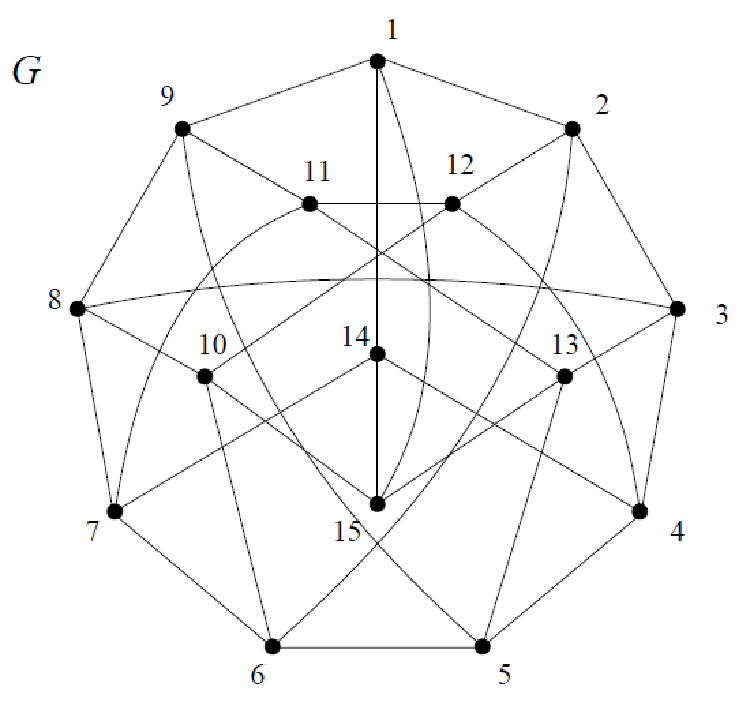
\includegraphics[scale=0.5]{media/4regdiam2on15}
%\caption{Potential $4$-regular graph with diameter $2$ on $15$ vertices.}\label{fig:4regdiam2on15}
%\end{center}
%\end{figure}
\end{multicols}
\vspace{2em}
\noindent \underline{\hspace{5in}}
\newpage
\vspace{2em}
\noindent{\bf \maltese \hspace{1em} Sub-Experience Three: Non-Standard Dice}\\
\noindent(\emph{No outside resources, please.}) A 6-sided die labeled with the integers $1, 2, 3, 4, 5, 6$ will be called a \emph{standard die}.  The goal for this part of the \emph{Final} Experience is to determine all ways to label a pair of dice with positive integers so that the probabilities of rolling the usual sums $2, 3, \dots ,12$ are the same, but the labels are non-standard.  \\
\noindent{\bf Step 1.}  Let $p(x) = x+x^2+x^3+x^4+x^5+x^6$, and explain why $(p(x))^2$ is the generating function for the probabilities of outcomes in rolling a pair of standard dice.\\
\noindent{\bf Step 2.}  Let $A =(a_1, a_2, a_3, a_4, a_5, a_6)$ and $B = (b_1, b_2, b_3, b_4, b_5, b_6)$ be two lists of positive integers.  Put $p_A(x) = x^{a_1}+x^{a_2} + x^{a_3} + x^{a_4}+x^{a_5} + x^{a_6}$ and $p_B(x) = x^{b_1}+x^{b_2}+x^{b_3}+x^{b_4}+x^{b_5}+x^{b_6}$.  Explain why finding $a_i$s and $b_i$s such that $p_A(x)p_B(x) = (p(x))^2$ is relevant this part of the Experience.\\
\noindent{\bf Step 3.}  Factor $p(x)$ into irreducible polynomials and use this factorization to help solve for the $a_i$s and $b_i$s. Specifically, the factorization will force the form of $p_A(x)$ to be something like $p_1(x)^qp_2(x)^rp_3(x)^sp_4(x)^t$, where $0 \leq q,r,s,t \leq 2$ and $p_i(x)$, for $1 \leq i \leq 4$, is a factor of $p(x)$.  In your solution to this step, you must motivate why you take this step. \\
\noindent{\bf Step 4.} Begin to reduce the possibilities for $q,r,s,$ and $t$ by using information from $p_A(1)$ and $p_A(0)$.  Note that, on one hand $p_A(1) = 1^{a_1} + 1^{a_2} + 1^{a_3} + 1^{a_4} + 1^{a_5}+1^{a_6} = 6$ (since $a_i > 0$), and on the other hand we have $p_A(1) = p_1(1)^qp_2(1)^rp_3(1)^sp_4(1)^t$.  Similarly, there are two ways to view $p_A(0)$.\\
\noindent{\bf Step 5.} List all possible ways to label a pair of dice so that the probabilities of obtaining the sums $2, 3, 4, 5, 6, 7, 8, 9$, $10, 11, 12$ are $\frac{1}{36}, \frac{2}{36}, \frac{3}{36}, \frac{4}{36}, \frac{5}{36}, \frac{6}{36}, \frac{5}{36}, \frac{4}{36}, \frac{3}{36}, \frac{2} {36},\frac{1}{36}$, respectively.  One such way will be the standard way.  In your solution for this step, explain why you have proved that the labels you have found are the only possible ones that give the desired probabilities for roll- outcomes.
\vspace{2em}
\noindent \underline{\hspace{5in}}
\vspace{2em}
\noindent{\bf \maltese \hspace{1em} Sub-Experience Four: Space Station Security}\\
\noindent(\emph{No outside resources, please}) We have defined space stations, and developed notation in class, in particular see \emph{Meeting Thirty-Three}.  Please use that notation in your responses to these prompts.  To remind: $S_w$ denotes a (specific) $w$-walled station, $\oint S_w$ denotes its interior, $\partial S_w$ denotes its boundary (its walls and corners).  Let's use $V(S_w)$ to denote the corners of $S_w$ and $W(S_w)$ to denote its walls.\\
\begin{enumerate}
	\item {\bf Watched Eyes.} The function $gg(w)$ is the maximum number of robot eyes (REs) required to protect any $w$-walled station which can be seen by at least one other RE.  Please make a conjecture for the value of $gg(w)$.  The points you earn from your response (your conjecture) will be proportional to the type and quantity of justification you give.  
	\item {\bf Rectangular Stations.}  Define the function $g_{\perp}(w)$ to be the maximum number of REs required to protect a $w$-walled station whose interior angles between walls are each either $90^{\circ}$ or $270^{\circ}$.  Please find the value for $g_{\perp}(w)$ and prove the value you find is correct.
	\item {\bf Watched Eyes in Rectangular Stations.} Define the function $gg_{\perp} (w)$ to be the maximum number of REs required to protect a $w$-walled rectangular station such that each RE can be seen by at least one other RE. Please determine the value for $gg_{\perp}(w)$ and prove the value is correct.
\end{enumerate}
\noindent \underline{\hspace{5in}}
\end{document}
